\chapter{System Design of Chess App}
\label{cha:design}

\section*{Introduction of System Design}
This section presents the detailed architectural design of \textbf{Guardians of the Chess Grandmaster (GOTCG)}, a web application platform designed to challenge and train players to think like a grandmaster. The design follows a client-server architecture with a React-based \texttt{frontend} and Node.js/Express \texttt{backend}, integrated with both Firebase and MongoDB for authentication, real-time data, and game analytics.

The architecture has been informed by the technology review conducted in the previous section, emphasizing scalability, real-time communication, and a responsive user experience across devices.

\section{Overall System Architecture}
\subsection*{System Architecture Diagram}
The system follows a modern full-stack web architecture, with a clear separation of concerns across the \texttt{frontend}, \texttt{backend}, and data layers. The \texttt{frontend} is responsible for user interaction and presentation, providing a responsive and dynamic user interface. The \texttt{backend} manages core application logic, authentication, and real-time communication between clients. Data persistence is handled using both Firebase and MongoDB, with each technology serving different requirements depending on the use case. This hybrid approach enables efficient user management alongside scalable storage for game state and analytics data. Here's an example from Figure~\ref{fig:sysad}

\begin{figure}
    \centering
    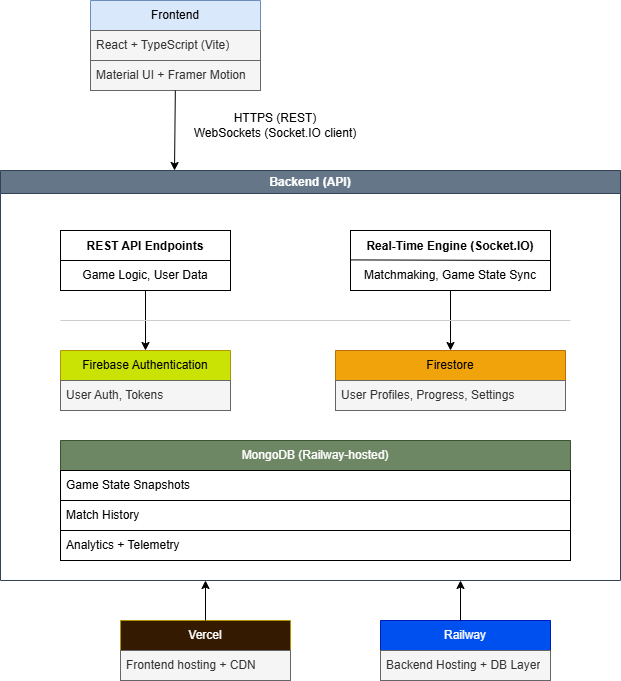
\includegraphics[width=0.5\linewidth]{images//System Architecture Diagram/MyArchitecture.png}
    \caption{My System Architecture Diagram}
    \label{fig:sysad}
\end{figure}

\subsection*{High-Level Architecture}
The GOTCG platform employs a \textbf{three-tier architecture}:
\begin{enumerate}
    \item \textbf{Presentation Layer}: React SPA (Single Page Application) with TypeScript
    \item \textbf{Application Layer}: Node.js/Express API server with Socket.IO for real-time features
    \item \textbf{Data Layer}: Dual database strategy - Firebase (authentication \& Firestore) + MongoDB (game data \& analytics)
\end{enumerate}

\subsection*{Component Coupling \& Communication Standards}
\subsubsection*{Standards-Based Integration}

\begin{itemize}
    \item \textbf{REST API}: HTTP/HTTPS communication between \texttt{frontend} and \texttt{backend}
    \item \textbf{WebSocket Protocol}: Socket.IO for bi-directional real-time communication
    \item \textbf{JSON Data Format}: All API payloads use JSON for data interchange
    \item \textbf{Firebase SDK}: Official Firebase client library for authentication
    \item \textbf{Mongoose ODM}: Object-Document Mapping for MongoDB schemas
\end{itemize}

\subsubsection*{Component Coupling}

\begin{itemize}
    \item \textbf{Frontend $\leftrightarrow$ Backend}: Loosely coupled via REST API contracts and WebSocket events
    \item \textbf{Backend $\leftrightarrow$ Databases}: Abstracted through configuration modules $\newline$(\texttt{/backend/src/config/})
    \item \textbf{State Management}: React Context API for global state (Auth, Theme, Board Theme)
\end{itemize}

\section{Detailed Component Design}

\subsection*{Frontend Architecture (Presentation Layer)}

\subsubsection*{Technology Stack}

The \texttt{frontend} is built using modern web technologies as defined in Table~\ref{tab:tsf}

\begin{table}
    \centering
    \newcolumntype{s}{>{\columncolor[HTML]{AAACED}} l}
    \newcolumntype{t}{>{\columncolor[HTML]{FF0000}} l}
    \begin{tabular}{|s|t|}
        \hline
        \textbf{Technology} & \textbf{Purpose} \\ \hline
        React & Language \\ \hline
        TypeScript & Application framework \\ \hline
        Vite & Authentication \& authorisation \\ \hline
        Firebase & Database access (Hibernate) \\ \hline
        HTML & Relational database \\ \hline
        CSS & Stateless auth tokens \\ \hline
    \end{tabular}
    \caption{Technology Stack from \texttt{frontend}}
    \label{tab:tsf}
\end{table}

\subsubsection*{Frontend Structure}

The \texttt{frontend} follows a layered architecture pattern following this link and looks for \texttt{Project Structure} \href{https://github.com/tomaspettit2506/final-year-project/blob/main/frontend/README.md}{GOTCG Frontend Project Structure}

\subsubsection*{Key Frontend Components}

The main application component (\texttt{App.tsx}) implements route-based navigation with authentication guards \href{https://github.com/tomaspettit2506/final-year-project/blob/main/frontend/src/App.tsx}{Route Configuration}

\subsubsection*{Firebase Integration}

Firebase is configured for authentication and Firestore database access \href{https://github.com/tomaspettit2506/final-year-project/blob/main/frontend/src/firebase.ts}{Firebase Configuration}

\subsubsection*{State Management Pattern}

The application uses React Context API for global state management with a hierarchical provider structure \href{https://github.com/tomaspettit2506/final-year-project/blob/main/frontend/src/main.tsx}{Context Provider Hierarchy}

This pattern ensures:
\begin{itemize}
    \item \textbf{AuthProvider}: Manages user authentication state
    \item \textbf{ThemeProvider}: Handles light/dark theme preferences
    \item \textbf{BoardThemeProvider}: Controls chess board appearance
\end{itemize}

\subsection*{Backend Architecture (Application Layer)}

\subsubsection*{Technology Stack}

The \texttt{backend} leverages Node.js with the following table on Table~\ref{tab:tsb}


\begin{table}
    \centering
    \newcolumntype{s}{>{\columncolor[HTML]{AAACED}} l}
    \newcolumntype{t}{>{\columncolor[HTML]{FF0000}} l}
    \begin{tabular}{|s|t|}
        \hline
        \textbf{Technology} & \textbf{Purpose} \\ \hline
        Node.js & Runtime environment \\ \hline
        TypeScript & Language \\ \hline
        Express.js & Web framework \\ \hline
        MongoDB (via Mongoose) & Database \\ \hline
        Firebase Admin SDK & Authentication \& notifications \\ \hline
        Jest & Testing framework \\ \hline
        Docker & Containerization (optional, for deployment) \\ \hline
    \end{tabular}
    \caption{Technology Stack from \texttt{backend}}
    \label{tab:tsb}
\end{table}

\subsubsection*{Backend Structure}

The \texttt{backend} follows a layered architecture pattern following this link and look for \texttt{Project Structure} \href{https://github.com/tomaspettit2506/final-year-project/blob/main/backend/README.md}{GOTCG Backend Project Structure}

\subsubsection*{Server Configuration}

The server entry point (\texttt{index.ts}) configures Express, CORS, and Socket.IO \href{https://github.com/tomaspettit2506/final-year-project/blob/main/backend/src/index.ts}{Server Configuration}

\subsubsection*{API Endpoint Structure}

The RESTful API exposes the following endpoint hierarchy \ref{table:api-endpoints}:

\begin{table}[ht]
\centering
\newcolumntype{s}{>{\columncolor[HTML]{AAACED}} p{3.5cm}}
\newcolumntype{t}{>{\columncolor[HTML]{FF0000}} p{2cm}}
\newcolumntype{u}{>{\columncolor[HTML]{3CB371}} p{4cm}}
\begin{tabular}{|s|t|u|}
\hline
\rowcolor{lightgray} \multicolumn{3}{|c|}{API Endpoint Reference} \\ \hline
\textbf{Endpoint} & \textbf{Method} & \textbf{Description} \\ \hline
\texttt{/user/:id} & GET & Get user profile \\ \hline
\texttt{/user} & POST & Create user \\ \hline
\texttt{/user/:id} & PUT & Update user \\ \hline
\texttt{/game/:id} & GET & Get game details \\ \hline
\texttt{/game} & POST & Create new game \\ \hline
\texttt{/game/:id} & PUT & Update game state \\ \hline
\texttt{/friend/:userId} & GET & Get friends list \\ \hline
\texttt{/friend/add} & POST & Send friend request \\ \hline
\texttt{/friend/:friendId} & DELETE & Remove friend \\ \hline
\texttt{/game-invite/:id} & GET & Get game invites \\ \hline
\texttt{/game-invite} & POST & Send game invite \\ \hline
\texttt{/request/:userId} & GET & Get pending requests \\ \hline
\texttt{/request/respond} & POST & Accept/reject request \\ \hline
\texttt{/message/:chatId} & GET & Get chat messages \\ \hline
\texttt{/message} & POST & Send message \\ \hline
\end{tabular}
\caption{API Endpoint Reference}
\label{table:api-endpoints}
\end{table}

\subsection*{Data Layer Architecture}

\subsubsection*{Dual Database Strategy}

The system employs two complementary database systems:

\begin{enumerate}
    \item \textbf{Firebase (Authentication \& Real-time Data)}
    \begin{itemize}
        \item \textbf{Firebase Authentication}: Email/password + Google Sign-In
        \item \textbf{Firestore}: User profiles, preferences, achievements
        \item \textbf{Use Case}: User authentication, session management
    \end{itemize}

    \item \textbf{MongoDB (Game Data \& Analytics)}
    \begin{itemize}
        \item \textbf{Connection}: MongoDB Atlas cloud-hosted
        \item \textbf{Use Case}: Game states, move history, analytics, statistics
    \end{itemize}
\end{enumerate}

\section{Real-Time Communication (Socket.IO)}

\subsection*{WebSocket Event Handlers}

Socket.IO manages real-time bidirectional communication for:

\begin{itemize}
    \item \textbf{Game Moves}: Broadcasting chess moves to both players
    \item \textbf{Game Invitations}: Real-time friend game invites
    \item \textbf{Chat Messages}: In-game messaging
    \item \textbf{Room Management}: Creating/joining game rooms
\end{itemize}

\subsection*{Room-Based Architecture}

The \texttt{backend} maintains a room-based structure for game sessions, allowing one player to create a Room ID (six random digits), and when another player joins the same Room ID, it is the same as Player 1's.

\subsection*{Socket Events}
\begin{itemize}
    \item \textbf{Client → Server Events:} This enables the client to join a game room, send chess moves, chat with friends, and leave the game room if they have checkmated an opponent, resigned, timed out, or abandoned the game. Refer to Table~\ref{table:socket-client-server} for examples.
    \item \textbf{Server → Client Events:} This allows the server to notify the client about game creation, broadcast moves to the opponent (client), share chat messages with friends, and notify the client of the game's conclusion. Refer to Table~\ref{table:socket-server-client} for examples.
\end{itemize}

\begin{table}[ht]
\centering
\newcolumntype{s}{>{\columncolor[HTML]{AAACED}} l}
\newcolumntype{t}{>{\columncolor[HTML]{FF0000}} l}
\begin{tabular}{|s|t|}
\hline
\rowcolor{lightgray} \multicolumn{2}{|c|}{\textbf{Client → Server Events}} \\ \hline
\textbf{Event} & \textbf{Description} \\ \hline
joinRoom & Join a game room \\ \hline
makeMove & Send chess move \\ \hline
sendMessage & Send chat message \\ \hline
leaveRoom & Leave game room \\ \hline
\end{tabular}
\caption{Client to Server Socket Events}
\label{table:socket-client-server}
\end{table}

\begin{table}[ht]
\centering
\newcolumntype{s}{>{\columncolor[HTML]{AAACED}} l}
\newcolumntype{t}{>{\columncolor[HTML]{FF0000}} l}
\begin{tabular}{|s|t|}
\hline
\rowcolor{lightgray} \multicolumn{2}{|c|}{\textbf{Server → Client Events}} \\ \hline
\textbf{Event} & \textbf{Description} \\ \hline
gameCreated & Notify game creation \\ \hline
moveMade & Broadcast move to opponent \\ \hline
messageReceived & Broadcast chat message \\ \hline
gameEnded & Notify game conclusion \\ \hline
\end{tabular}
\caption{Server to Client Socket Events}
\label{table:socket-server-client}
\end{table}

\section{Cloud Infrastructure \& Deployment}

\subsection*{Development Environment}

\begin{itemize}
    \item \textbf{Frontend}: Vite dev server (Ports 5173, 5174, 5175 for multi-instance testing)
    \item \textbf{Backend}: Node.js with nodemon (Ports 8000, 8001, 8002)
\end{itemize}

\subsection*{Database Hosting}

\begin{itemize}
    \item \textbf{Firebase}: Google Cloud Platform (GCP) - Authentication, Firestore
    \item \textbf{MongoDB}: MongoDB Atlas (Cloud-hosted DBaaS)
\end{itemize}

\subsection*{Progressive Web App (PWA)}

The application leverages \texttt{vite-plugin-pwa} for:

\begin{itemize}
    \item Offline support through service worker caching
    \item Installation to device home screen
    \item Native app-like experience across platforms
    \item Notifications allow apps to send alerts to users even when the app is closed. For example, send or reply a message and send a request to be a friend
\end{itemize}

\subsection*{Deployment Strategy (SaaS/PaaS)}
To deploy a SaaS application using Vercel for the \texttt{frontend} and Railway for the \texttt{backend} ({\color{orange}{Warning:}} the \texttt{backend} should not be deployed to Vercel because Socket.IO/WebSocket support is required), consider the following steps:
\begin{enumerate}
    \item \textbf{Vercel:}
    \begin{itemize}
        \item Host the \texttt{frontend} on Vercel, which is optimized for Next.js and other frameworks. It offers features like serverless functions, global CDN, and easy deployment via Git integration.
        \item Use Vercel's deployment hooks for automated deployments and preview URLs for testing.
    \end{itemize}
    
    \item \textbf{Railway:}
    \begin{itemize}
        \item Deploy the \texttt{backend} on Railway, which is a container-focused PaaS that supports various frameworks and offers predictable billing.
        \item Utilize Railway's features like one-click deploys and built-in database support for full-stack applications.
    \end{itemize}
\end{enumerate}

\section*{Security Design}

\subsection*{Authentication \& Authorization}

\begin{itemize}
    \item \textbf{Firebase Authentication}: JWT-based token authentication
    \item \textbf{Google OAuth 2.0}: Third-party authentication provider
    \item \textbf{CORS Configuration}: Whitelist of allowed origins
\end{itemize}

\subsection*{Data Security}

\begin{itemize}
    \item Environment variables for sensitive credentials (\texttt{.env} files)
    \item HTTPS/TLS for all production traffic
    \item Firebase Admin SDK for server-side authentication verification
    \item Password hashing handled by Firebase Authentication
\end{itemize}

\section*{Design Rationale}

The architecture choices were informed by the technology review conducted in the previous chapter. Key decisions include \ref{table:tech-rationale}:

\begin{table}[!ht]
\centering
\newcolumntype{s}{>{\columncolor[HTML]{AAACED}} p{5cm}}
\newcolumntype{t}{>{\columncolor[HTML]{FFF332}} p{10cm}}
\begin{tabular}{|s|t|}
\hline
\textbf{Technology} & \textbf{Rationale} \\ \hline
React + TypeScript & Type safety, component reusability, modern development experience \\ \hline
Vite & Fast HMR (Hot Module Replacement), optimized production builds \\ \hline
Material-UI & Consistent, accessible UI components following Material Design principles \\ \hline
Socket.IO & Cross-browser WebSocket support with automatic fallback mechanisms \\ \hline
Firebase & Scalable authentication, real-time database capabilities, managed infrastructure \\ \hline
MongoDB & Flexible schema for complex game data, excellent query performance for analytics \\ \hline
Node.js/Express & JavaScript full-stack development, extensive ecosystem, event-driven architecture \\ \hline
PWA & Offline capabilities, native app-like experience, cross-platform compatibility and notification \\ \hline
\end{tabular}
\caption{Technology Selection Rationale}
\label{table:tech-rationale}
\end{table}

\subsection*{Scalability Considerations}

The chosen architecture supports horizontal scaling through:

\begin{itemize}
    \item \textbf{Stateless Backend}: Express servers can be replicated without session affinity
    \item \textbf{Socket.IO Redis Adapter}: Enables WebSocket connection sharing across multiple server instances
    \item \textbf{Cloud Databases}: Firebase and MongoDB Atlas automatically scale with demand
    \item \textbf{CDN Distribution}: Static \texttt{frontend} assets served globally through CDN
\end{itemize}

\subsection*{Performance Optimization}

Performance is optimized through:

\begin{itemize}
    \item \textbf{Code Splitting}: React lazy loading for route-based components
    \item \textbf{Service Worker Caching}: PWA caches static assets for faster subsequent loads
    \item \textbf{Database Indexing}: MongoDB indexes on frequently queried fields (\texttt{userId}, \texttt{gameId})
    \item \textbf{WebSocket Compression}: Socket.IO compression reduces message payload sizes
\end{itemize}

\section*{Conclusion}

This system design presents a comprehensive, scalable architecture for the \textit{GOTCG} platform. The three-tier architecture with dual database strategy balances real-time requirements (Firebase) with complex data analytics needs (MongoDB). The use of modern web standards (REST, WebSocket, OAuth 2.0) ensures compatibility and maintainability, while the PWA approach provides a native-like experience across devices.

The design has been validated through implementation, as evidenced by the running codebase in the \texttt{tomaspettit2506/final-year-project} repository. Future enhancements could include AI-powered move suggestions, tournament management systems, and advanced analytics dashboards for player improvement tracking.